\setchapterimage[6cm]{chapter/operating_system/logo.png}
\setchapterpreamble[u]{\margintoc}
\chapter[Operating systems]{\mbox{Programming languages for operating systems\protect\footnotemark}}
\labch{operating-sysmets}

\footnotetext{Ubuntu 19.04 ``Disco Dingo'' Author: \href{https://commons.wikimedia.org/wiki/File:Ubuntu_19.04_\%22Disco_Dingo\%22.png}{JulianVilla26 / 2019 / GNU General Public License}.}

This chapter explores the Wikidata object ``operating system'' and its properties. In each of the sections, tasks are presented that were solved using SPARQL queries. Among them: finding instances of the object ``operating system'', building lists of operating systems (OS) containing information about their ``ancestors'' (operating systems that served as the basis for creating a new one), the time of their creation, the programming languages in which the OS was written.
A histogram is also built showing the number of programs written in a particular programming language, and what proportion of them work under a particular OS. 
For a large number of operating systems, Wikidata does not indicate the programming language in which it was developed, namely, for 2020, this property is indicated for only 29\% of the total number of systems.
Wikidata plays a big role in software documentation. But at the same time, Wikidata is filling up rapidly and plays a big role in software documentation.

\section{List of operating systems}

Listing \ref{lst:all_operating_systems} shows a SPARQL query to get the list of operating systems

\begin{lstlisting}[ language=SPARQL, 
caption={List of operating systems\\\hspace{\textwidth} 
SPARQL query \num{510} operating systems in 2018, \num{1086} in 2020.
SPARQL query: \href{https://w.wiki/nDb}{https://w.wiki/nDb}
},
label=lst:all_operating_systems,
texcl 
]
SELECT ?os ?osLabel
WHERE
{
	?os wdt:P31 wd:Q9135. # instance of operating system
SERVICE wikibase:label { bd:serviceParam wikibase:language "en" }
}
\end{lstlisting}

The most complete and well-developed operating systems on Wikidata are: \wdqName{Microsoft Windows}{1406} \wdqName{Windows 8}{5046}, \wdqName{GNU}{44571}, \wdqName{Windows 10}{18168774} 24 filled properties\cite{prowd_os_link}.

Almost empty and uninformative operating systems turned out to be: \wdqName{Novell DOS}{3345389}, \wdqName{MagiC}{1884068}, \wdqName{KallistiOS}{1722492}, and others. These systems have only one filled property\cite{prowd_os_link}.

According to ProWD, the only Russian operating system in Wikidata \wdqName{Miraculix}{4044344} has seven filled properties\cite{prowd_os_link_ru}.

\section{Operating systems bases}
Listing \ref{lst:base_of_operating_systems} shows a SPARQL query to get the list of \href{https://www.wikidata.org/wiki/Property_talk:P144}{based (P144)} operating systems. This query shows the correspondence between the \wdqName{operating system}{9135} and its ``ancestor'', that is, the previous operating system on which it is based.

\marginnote[-3.0cm]{
	Choose operating system 
	\href{https://w.wiki/n8U}{Debian},
	\href{https://w.wiki/n8V}{Android},
	\href{https://w.wiki/n8W}{Ubuntu} or
	\href{https://w.wiki/n8X}{Linux kernel}
	which has the most count of based on it other operating systems. \\
	See answer~\ref{answer:os_base} on page~\pageref{answer:os_base}. 
}

\begin{lstlisting}[ language=SPARQL, 
caption={List of operating systems by base\\\hspace{\textwidth}
SPARQL query \num{159} operating systems with bases in 2018, \num{118} in 2020.
SPARQL query: \href{https://w.wiki/vHZ}{https://w.wiki/vHZ}
},
label=lst:base_of_operating_systems,
texcl 
]
SELECT ?os ?osLabel ?base ?baseLabel
WHERE
{
	?os wdt:P31 wd:Q9135.
	?os wdt:P144 ?base.
SERVICE wikibase:label { bd:serviceParam wikibase:language "en" }
}
\end{lstlisting}

\section{Operating systems release dates}
\marginnote[-0.5cm]{
	Which of operating systems
	\href{https://w.wiki/n8P}{Newton OS},
	\href{https://w.wiki/n8Q}{Ubuntu Touch} or
	\href{https://w.wiki/n8R}{JavaOS} is developed by
	\href{https://w.wiki/n8S}{Apple}?\\
	See answer~\ref{answer:what_system_created} on page~\pageref{answer:what_system_created}.
}

Listing \ref{lst:inception_time_of_operating_systems} shows a SPARQL query to get a list of operating systems with their creation date.

\index{SPARQL!hide!List of operating systems by release date}
\index{Chart!Timeline!Part of a timeline with operating system release dates from 1955 to 2020}
\begin{lstlisting}[ language=SPARQL, 
caption={List of operating systems by release date\\\hspace{\textwidth}
SPARQL query \num{30} operating systems with release date in 2018, \num{238} in (2020).
SPARQL query: \href{https://w.wiki/v5Z}{https://w.wiki/v5Z}
},
label=lst:inception_time_of_operating_systems,
texcl 
]
#defaultView:Timeline{"hide": "?when"}
SELECT DISTINCT ?os ?osLabel ?when (YEAR(?when) as ?date) ?pic
WHERE
{
	?os wdt:P31 wd:Q9135. # instance of operating system
	?os wdt:P571 ?when. # inception date
	OPTIONAL { ?os wdt:P18 ?pic }
SERVICE wikibase:label {bd:serviceParam wikibase:language "en"}
}
GROUP BY ?osLabel ?time
ORDER BY DESC(?time)
\end{lstlisting}

When creating a SPARQL query \ref{lst:inception_time_of_operating_systems}, the \{"hide": "?when"\} option was used for the \#defaultView:Timeline command.
\marginnote{The command \#defaultView:Timeline, which looks like a comment, is actually an instruction from the Wikidata Query Service (WDQS for short) so that the result is not presented as a table (by default), but on a timeline, see figure~\ref{lst:count_os_on_languages}}
This option allows the data to be used to create the appearance of the query, without directly displaying it \cite{WQSResultViews}.

Listing \ref{lst:inception_time_of_operating_systems} shows in a nice graphical shell (figure \ref{fig:os_creation}) the timeline of the creation (actually the release)
\marginnote[0.5cm]{Building an operating system is a lengthy process, often taking years. In this case, the date when the system was made publicly available is indicated.}
of operating systems. It also shows how poorly Wikidata is filled, since only \num{230} operating systems are displayed in requests (this is 21\% of the total) for 2020. Which, in turn, means that the creation date field for the remaining objects is simply not filled. Although the information about the release date is not so secret.

\begin{figure*}[h!]
	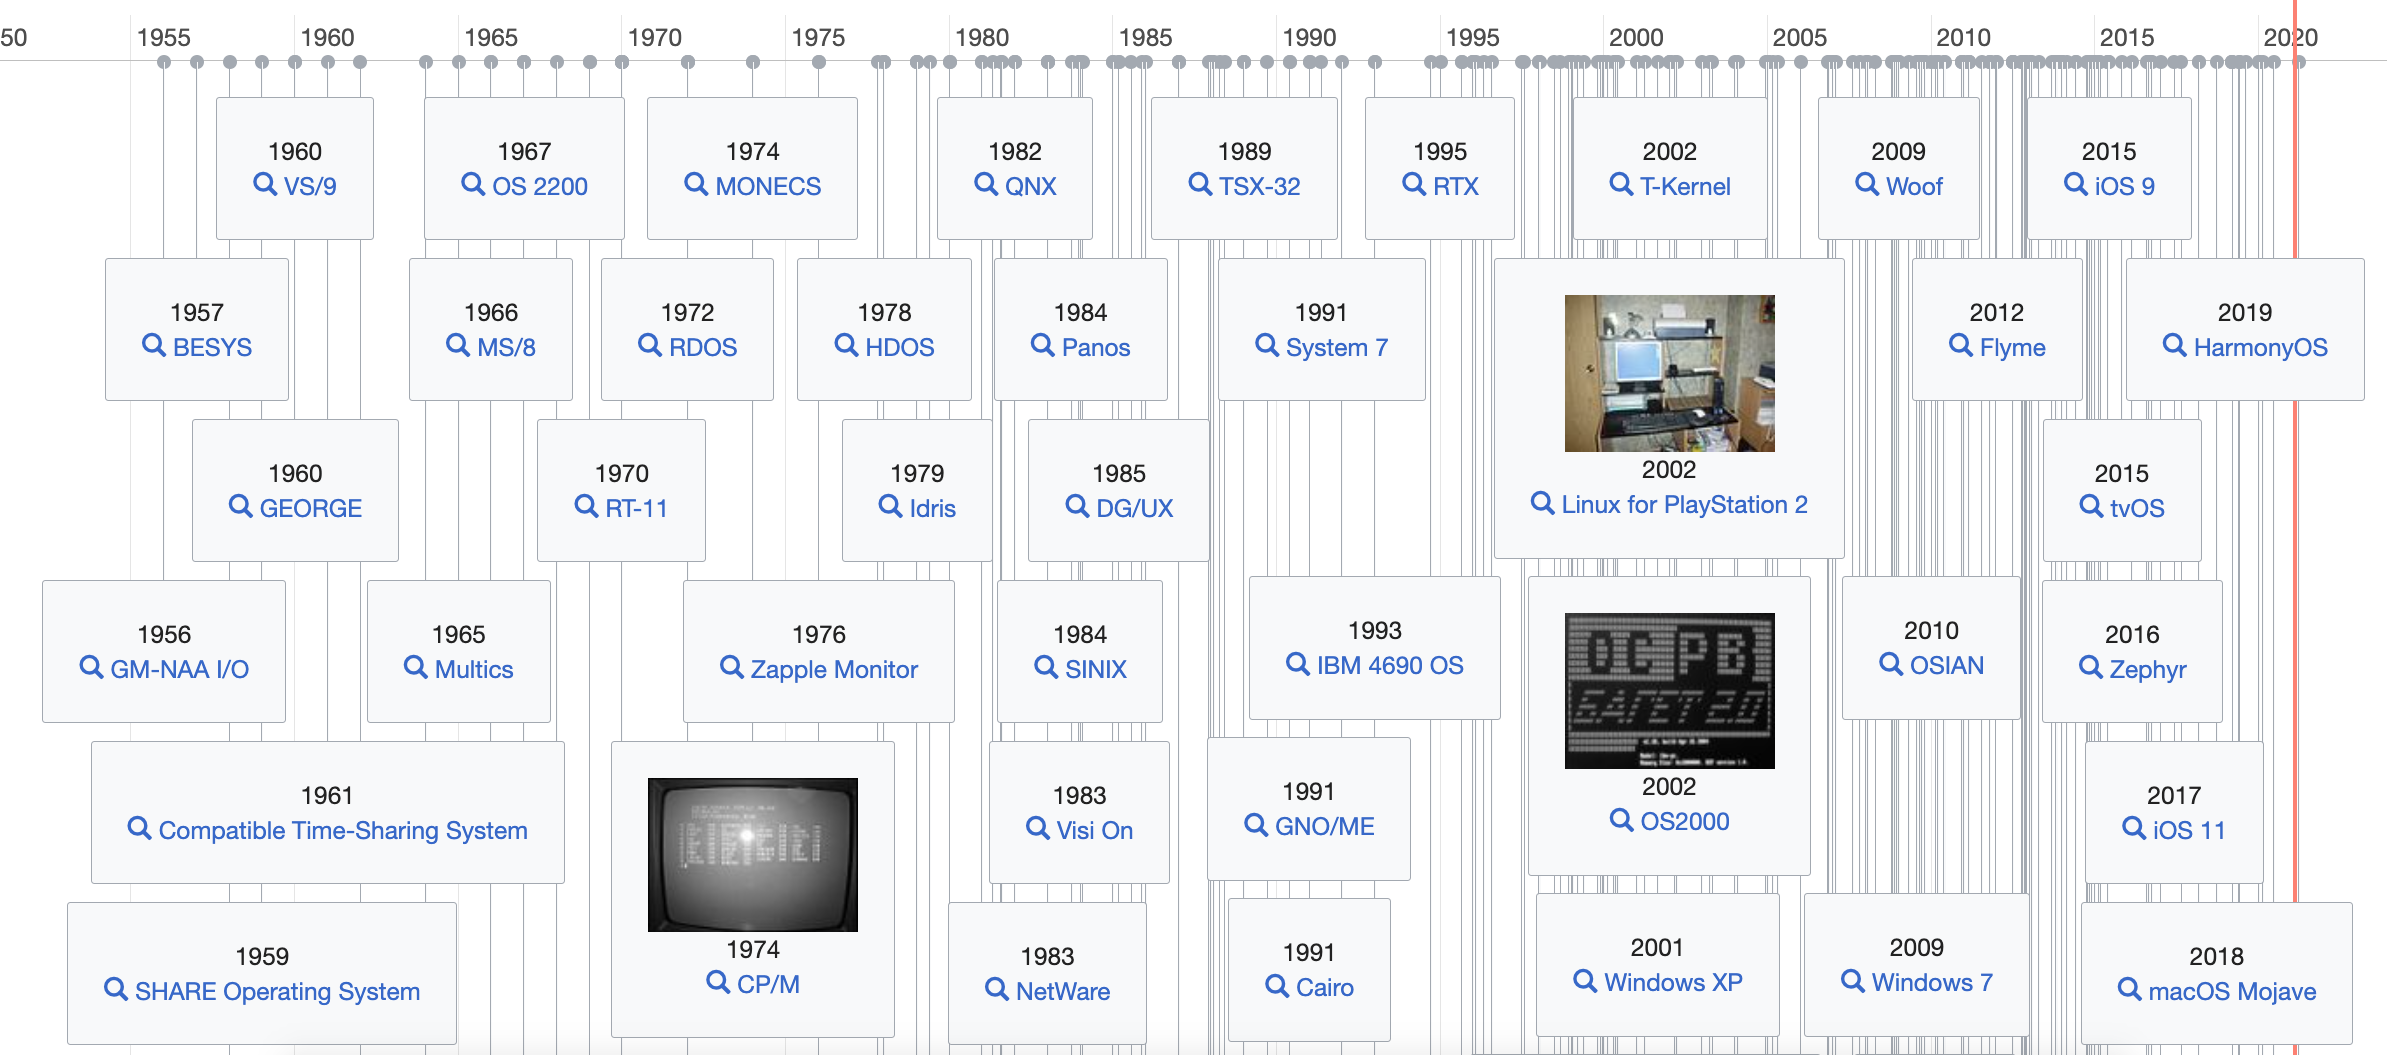
\includegraphics{./chapter/operating_system/os-creation.png}
	\caption{Part of a timeline with operating system release dates from 1955 to 2020}
	\label{fig:os_creation}
\end{figure*}

\section{Count of operating systems written in programming languages}

Listing \ref{lst:count_os_on_languages} shows a SPARQL query to get a list of programming languages with the output of the number of operating systems written in them.

\begin{lstlisting}[ language=SPARQL, 
caption={Count of operating systems by programming language\\\hspace{\textwidth}
SPARQL query \num{35} programming languages used to write operating systems in 2018), \num{37} in 2020.
SPARQL query: \href{https://w.wiki/vJN}{https://w.wiki/vJN}
},
label=lst:count_os_on_languages,
texcl 
]
# Languages and number of OS written in these languages
SELECT ?lang ?langLabel (COUNT(*) AS ?countOS)
WHERE 
{
	?os wdt:P31 wd:Q9135. # is instance of operating system
	?os wdt:P277 ?lang. # is written in programming language ?lang
SERVICE wikibase:label {bd:serviceParam wikibase:language "en"}
}
GROUP BY ?lang ?langLabel
ORDER BY DESC(?countOS) ASC(?langLabel)
\end{lstlisting}

The ORDER BY DESC(?countOS) ASC(?langLabel) command in the SPARQL query \ref{lst:count_os_on_languages} is used to double sort values in the table. All programming languages will be sorted in descending order by the count of operating systems written in them, and if their number is equal, they will be sorted in alphabetical order by name.

The result of the SPARQL query \ref{lst:count_os_on_languages} shows that mainly operating systems are written in C (46 operating systems) and assembler (42 operating systems). C ++ (16 operating systems) is in third place.

Using the SPARQL query \ref{lst:lang_tree}, you can get a diagram of programming languages and operating systems written in them in the form of a tree (figure~\ref{fig:prog_lang_os})

\marginnote[-5.5cm]{
	A difficult task for independent work. Modify the script \ref{lst:lang_tree} (\href{https://w.wiki/ucB}{https://w.wiki/ucB}) so that the number of operating systems written in this language.
}

\marginnote[-3.0cm]{
	A simple task for independent work. ``flip'' the script \ref{lst:lang_tree} (\href{https://w.wiki/ucB}{https://w.wiki/ucB}), that is, the top-level lines should not contain programming languages , but operating systems. When ``expanding'', we should see a list of languages in which the system is written.
}

\index{SPARQL!OPTIONAL!List of programming languages and operating systems written in them}
\index{Chart!Tree!The tree of programming languages and operating systems written in them}
\begin{lstlisting}[ language=SPARQL, 
caption={List of programming languages and operating systems written in them\\\hspace{\textwidth}
	SPARQL query \num{146} programming languages used to write operating systems in 2021.
	SPARQL query: \href{https://w.wiki/vJg}{https://w.wiki/vJg}
},
label=lst:lang_tree,
texcl 
]
# Languages and operating systems written in these languages
#defaultView:Tree
SELECT ?lang ?image ?logoImage ?langLabel 
?os ?osImage ?osLogoImage ?osLabel 
WHERE 
{
	?os wdt:P31 wd:Q9135. # is instance of operating system
	?os wdt:P277 ?lang. # is written in programming language ?lang
	OPTIONAL { ?lang wdt:P18 ?image. }
	OPTIONAL { ?lang wdt:P154 ?logoImage. }
	OPTIONAL { ?os wdt:P18 ?osImage. }
	OPTIONAL { ?os wdt:P154 ?osLogoImage. }
SERVICE wikibase:label {bd:serviceParam wikibase:language "en"}
}
\end{lstlisting}

\begin{marginfigure}[-4.0cm]
	{
		\setlength{\fboxsep}{0pt}%
		\setlength{\fboxrule}{1pt}%
		\fcolorbox{gray}{gray}{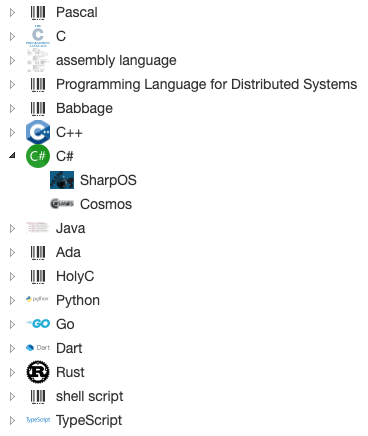
\includegraphics{chapter/operating_system/prog_lang_os.png}}
	}
	\caption{The tree of programming languages and operating systems written in them}
	\label{fig:prog_lang_os}
\end{marginfigure}

In this tree (figure~\ref{fig:prog_lang_os}), each line is a programming language. At the click of a mouse, you can expand a language and see a list of operating systems written using that language. If a language or system has a picture or logo on Wikidata, then they are used as icons.

\section{Data completeness}
According to the site www.operating-system.org there are 613 operating systems \cite{list_operating_systems}. While the Wikidata for 2017 contained information on only 510 operating systems (not including the \num{667} Linux distributions \cite{list_operating_systems}). And if you look at a large number of objects in the query results (the listings \ref{lst:inception_time_of_operating_systems} and \ref{lst:count_os_on_languages}), you will see that many objects are poorly filled, or even practically empty (for example, for \wdqName{Novell DOS}{3345389} and \wdqName{MagiC}{1884068} only one property \cite{prowd_os_link} is populated.).

In 2020, Wikidata contained information about 1086 operating systems (listing \ref{lst:all_operating_systems}), which indicates significant changes, namely, in three years (from 2017) the number of operating systems more than doubled from 510 to 1086. However, a large number objects are still poorly populated, for example, according to the query results \ref{lst:inception_time_of_operating_systems}, the release date information is filled only in \num{238} languages. From this we can conclude that Wikidata is incomplete, but filling up rapidly.

\section{Programming languages used to write operating systems}
If you look at the number of operating systems for which the property ``programming language'' is specified, you can see that out of \num{1086} objects this property is filled only in \num{116}. According to the data for 2020 (figure~\ref{fig:count-os-written-on-languages}) most of all operating systems, namely \num{44}, are written in the C programming language.

\begin{figure*}[h!]
	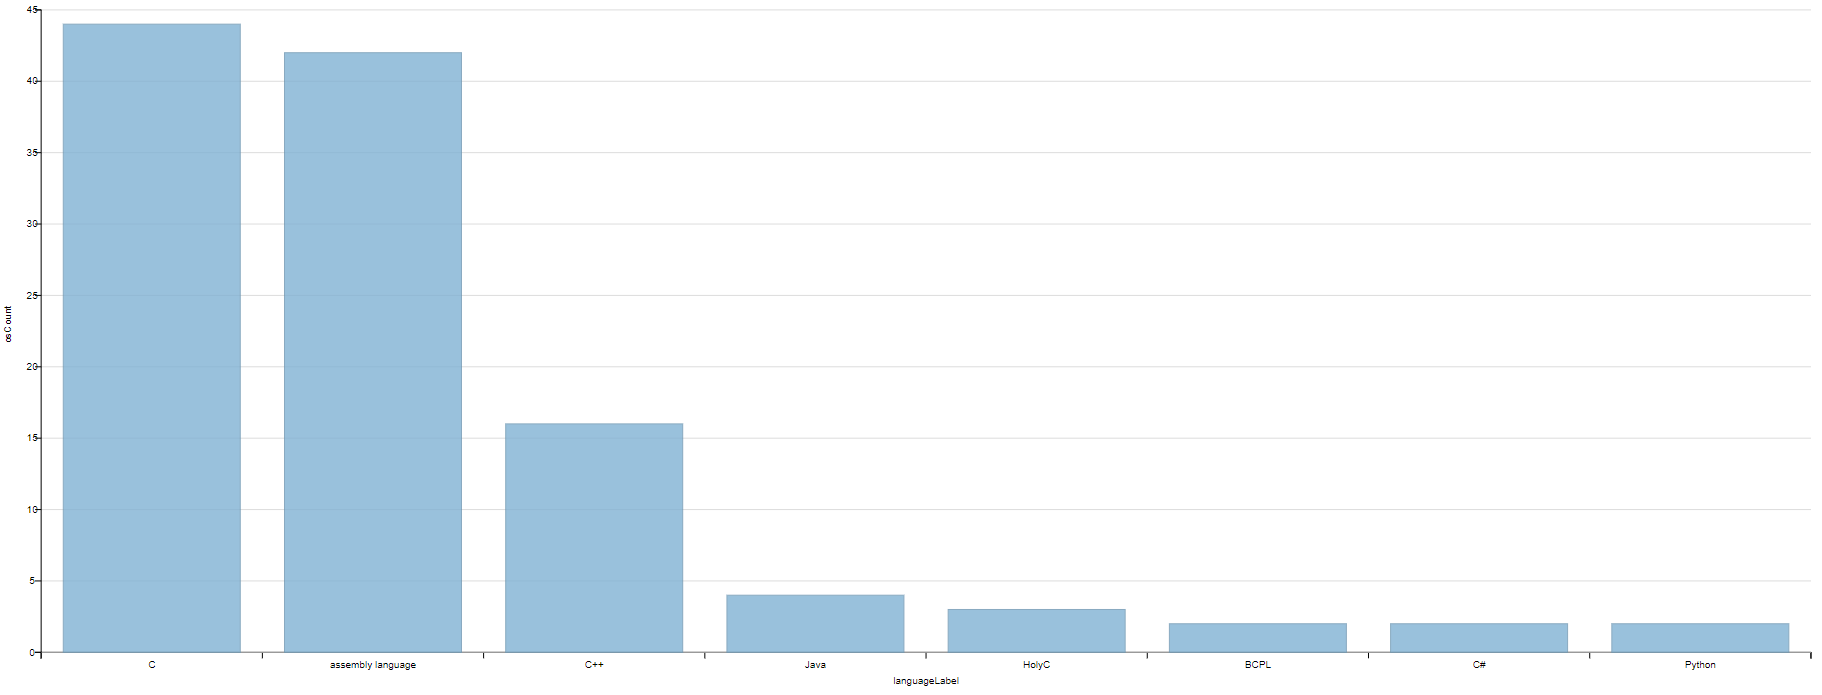
\includegraphics{./chapter/operating_system/count-os-written-on-languages.png}
	\caption{The first eight languages in which the most operating systems are written, 2020.}
	\label{fig:count-os-written-on-languages}
\end{figure*}

\section{Count of programs for each operating system}
Listing \ref{lst:count_soft_on_os} shows a SPARQL query showing how many programs are written for each operating system.

\begin{lstlisting}[ language=SPARQL, 
	caption={Count of programs for each operating system\\\hspace{\textwidth}
		\num{551} operating systems have programs written on it in 2020.
		SPARQL query: \href{https://w.wiki/vK3}{https://w.wiki/vK3}
	},
	label=lst:count_soft_on_os,
	texcl 
	]
# Number of software for each operating system
SELECT ?os ?osLabel (COUNT(*) AS ?softCounter)
WHERE
{ # the software ?soft works on the operating system ?os
	?soft p:P306 [ps:P306 ?os].
SERVICE wikibase:label { bd:serviceParam wikibase:language "en" }
}
GROUP BY ?os ?osLabel
ORDER BY DESC(?softCounter)
\end{lstlisting}

The leader among operating systems in terms by the count of programs written is \wdqName{Linux}{388}, for which \num{9223} programs have been written. For  \wdqName{Microsoft Windows}{1406} and  \wdqName{AIX}{269856} (unix operating system from \href{https://www.wikidata.org/wiki/Q37156}{IBM}) ware created  \num{3278} and \num{2337} programs.

\section{How much software was written for the OS using a particular language}
Listing \ref{lst:count_soft_on_os_with_lang} presents a SPARQL query showing for each software for each OS in how many languages it is written.

\begin{lstlisting}[ language=SPARQL, 
	caption={List of programming languages with the amount of software written for it\\\hspace{\textwidth}
		SPARQL query \num{704} computer programs were written for the operating system using one or another programming language, 2020.
		SPARQL query: \href{https://w.wiki/vKE}{https://w.wiki/vKE}
	},
	label=lst:count_soft_on_os_with_lang,
	texcl 
	]
#defaultView:BarChart
SELECT ?os ?osLabel (COUNT(*) AS ?softCount) 
?softLang ?softLangLabel
WHERE
{
	?soft wdt:P306 ?os. # software works on os
	?soft wdt:P277 ?softLang. # software is written by parogramming
	                           # language
	?os wdt:P277 ?osLang. # os is written by parogramming language
SERVICE wikibase:label { bd:serviceParam wikibase:language "en"}
}
GROUP BY ?os ?osLabel ?softLang ?softLangLabel
ORDER BY DESC(?count) DESC(?osLabel)
\end{lstlisting}

Request \ref{lst:count_soft_on_os_with_lang} perfectly shows that most of the software written for \href{https://www.wikidata.org/wiki/Q14116}{macOS} is written in \href{https://www.wikidata.org/wiki/Q2407}{C++} (374 programs), \href{https://www.wikidata.org/wiki/Q15777}{C} (276 programs), \href{https://www.wikidata.org/wiki/Q28865}{Python} (107 programs).
For \href{https://www.wikidata.org/wiki/Q94}{Android} written in \href{https://www.wikidata.org/wiki/Q2407}{C++} (107 programs) and \href{https://www.wikidata.org/wiki/Q251}{Java} (80 programs).
For \href{https://www.wikidata.org/wiki/Q48493}{iOS} written in \href{https://www.wikidata.org/wiki/Q2407}{C++} (63 programs).


The histogram in the figure~\ref{fig:count-software-written-on-languages} allows you to see for each programming language the number of programs that have been written in it, as well as under what OS these programs work. The graph shows that the largest number of programs is written in languages. \href{https://www.wikidata.org/wiki/Q2407}{C++} (2503 programs), 
\href{https://www.wikidata.org/wiki/Q15777}{C} (2566 programs), 
\href{https://www.wikidata.org/wiki/Q251}{Java} (799 programs),
\href{https://www.wikidata.org/wiki/Q28865}{Python} (717 programs),
\href{https://www.wikidata.org/wiki/Q2005}{Javascrip} (344 programs).


\begin{figure*}[h!]
	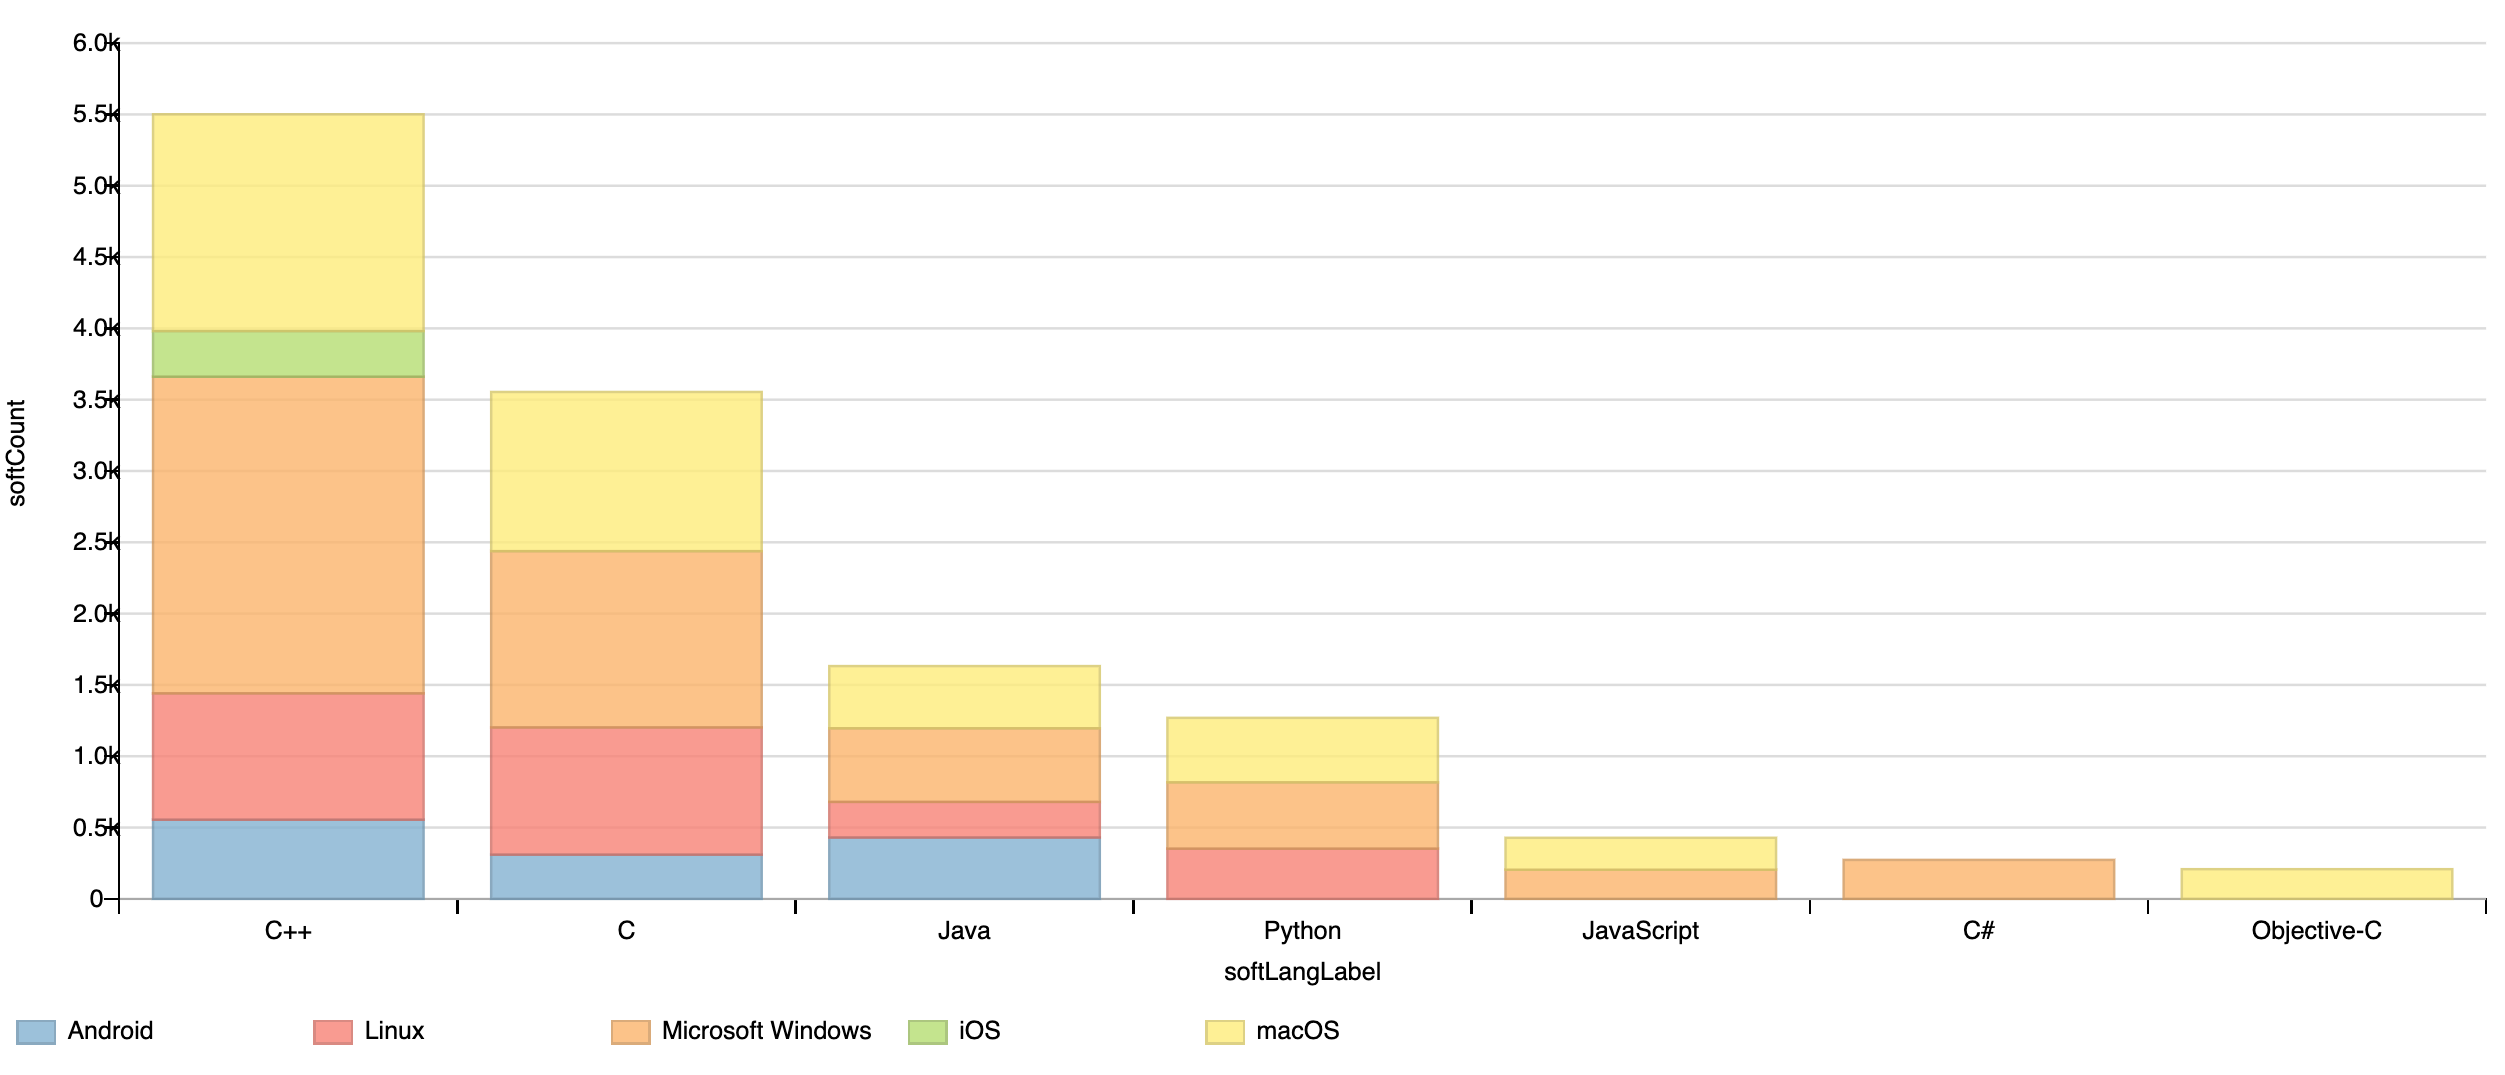
\includegraphics{./chapter/operating_system/Programming-languages-and-count-of-programms-written-on-them-and-OS-2020.png}
	\caption{Programming languages and the count of programs which for operating systems by these languages, 2020}
	\label{fig:count-software-written-on-languages}
\end{figure*}

Most of the C ++ programs are written for Windows (472 programs) and macOs (300 programs). Despite the fact that the C ++ language was developed in 1972, it has not yet lost its popularity due, probably, to the fact that it is used to write low-level applications.

Most C ++ programs are written for Windows (700 programs), macOS (400 programs), and Linux (400 programs). Probably, C ++ will lead for a long time, since at the moment it is used for solutions that require high performance, which is not allowed by a high-level language like Java \cite{Cilyurik2014LangPerformance}.

Most Java programs are written for macOS (196 programs) and Android (156 programs). Java is probably popular due to its code portability
\marginnote[-3.0cm]{Portability -- the ability to run code on multiple platforms without any changes}
that is, the Java code will run on any machine with the JVM installed
\marginnote[-2.0cm]{The Java virtual machine (JVM) -- runtime environment that can execute Java byte-code as a result of compiling computer programs written in the Java programming language}

Most JavaScript programs are written for macOS (100 programs), Android (60 programs) and iOS (40 programs). Typically, the language is used to write the client side of web applications.

Most Python programs are written for macOS (212 programs) and Linux (107 programs). The language is used, for example, to write web applications and analyze data.

Looking at the histogram (figure~\ref{fig:count-software-written-on-languages}), we can conclude that each of the languages considered has occupied its ``niche'' in the field of software development and is used for a certain range of tasks. Note that most of the software is written for macOS (900 programs), Windows (1500 programs), Linux (1200 programs) or Android (300 programs), as you can see from the script \ref{lst:count_soft_on_os}.

\section{Software Documentation}
Wikidata plays a big role in software documentation. This is illustrated by the programs included in the GNOME and KDE \cite{Samuel2020DocumentingWiki}. This article shows that while the English Wikipedia describes almost all the programs included in GNOME and KDE, the Italian and French ones only contain a subset of the articles. Documenting large projects is a well-known and difficult task. To solve it, you need a centralized system. It is in this role that the Wikipedia/Wikidata link acts\cite{Samuel2020DocumentingWiki}.

\section{Exercises}
\label{tasks:operating_system_tasks}
\begin{enumerate}
	\item Create list operating systems with information about their developers. The answer~\ref{answer:os_and_developers} can be found on the page~\pageref{answer:os_and_developers}.
	\item Find list operating systems with their logos. The answer~\ref{answer:os_and_logos} can be found on the page~\pageref{answer:os_and_logos}.
	\item Find countries of origin of operating systems. The answer~\ref{answer:os_country} can be found on the page~\pageref{answer:os_country}.
	\item Create a script that creates a tree diagram. Top-level lines should contain operating systems. When ``deploying'', we should see a list of operating systems that were based on the system from the top-level line. The answer~\ref{answer:os_and_bases} can be found on the page~\pageref{answer:os_and_bases}.
\end{enumerate}